

%% NOVAC
%% =============
%
In the following, I describe the technical implementation of the DOAS approach using the data of NOVAC instruments:\\
%
The first step is to correct each spectrum of the scan for dark current and offset using the dark spectrum.
The next task is to locate the spectra within and outside of the volcanic plume.
First a "pre-reference" (the spectrum recorded at an elevation angle of  0$^{\circ} $) is used to perform the evaluation of the scan spectra recorded at every elevation angle.
For every spectrum of the scan the \ce{SO2} differential slant column density (dSCD) with respect to the pre-reference is calculated using \Cref{eq:F} by the DOASIS fit routine.

The result is \ce{SO2} dSCDs as a function of the elevation angle. This way the elevation angle corresponding to the maximum and the minimum of the \ce{SO2} column density can be determined. The location of the \ce{SO2} maximum defines the location of the plume. The assumption is that the minimum of the \ce{SO2} curve corresponds to a region outside of the plume which is true in most cases. The background \ce{SO2} amount in the Earth's atmosphere around Tungurahua is usually negligible (see  \Cref{chap:so2}). \\
We use a gauss fit of the \ce{SO2}-elevation-angle-curve to define the plume region.
%
\begin{figure}
	\centering
	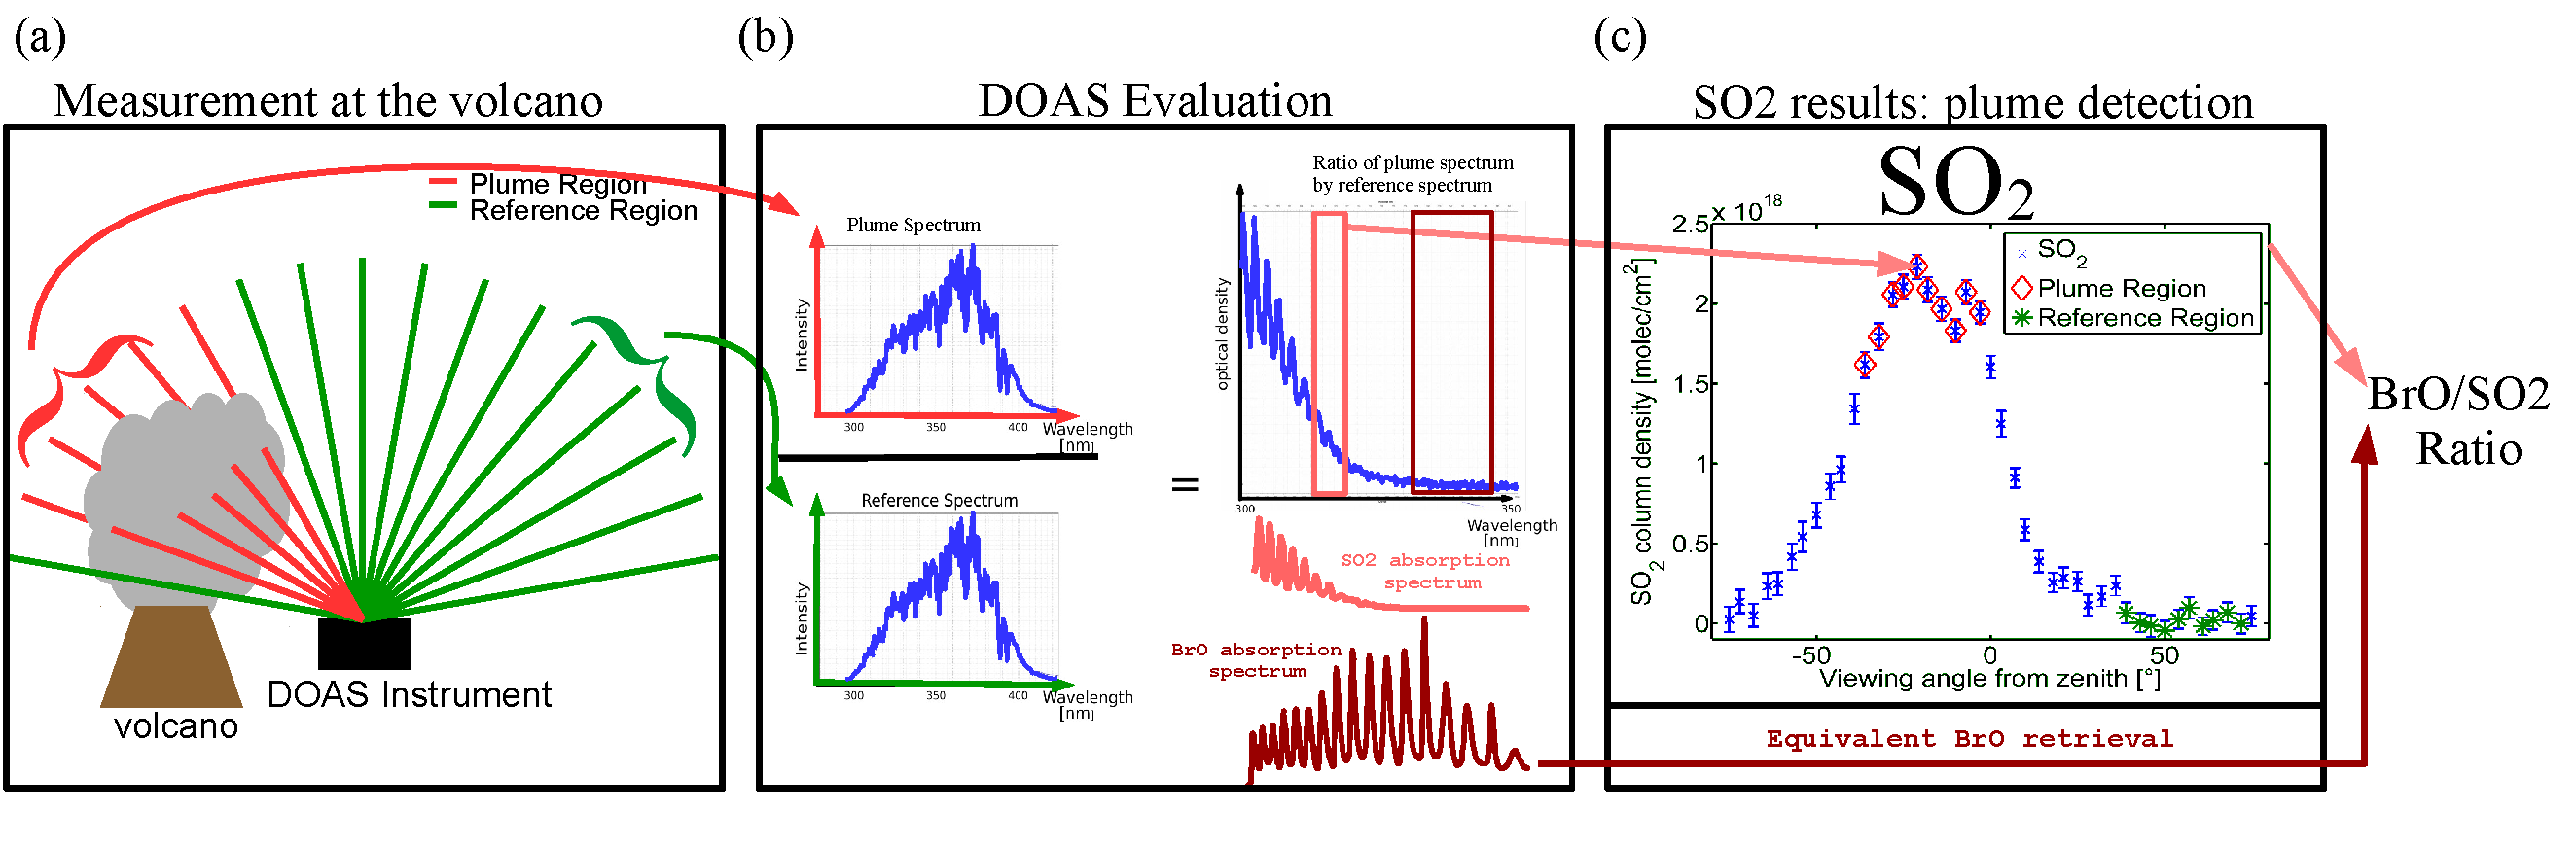
\includegraphics[width=1\linewidth]{Bilder/NOVAC_Eval}
	\caption{NOVAC evaluation: (a) Measurement at the volcano (b) Evaluation of the spectral data with the DOAS routine using the absorption cross sections of \ce{BrO}  and \ce{SO2}. (c) Finding the location of the plume and reference(taken from \cite{WarnachSimon}). With the so found plume and reference spectra, the BrO/\ce{SO2} can be calculated. }
	\label{fig:NOVAC_Eval}
\end{figure}
The sum over all plume spectra is taken, which are in the elevation angle interval of the gauss peak plus minus one sigma, to increase the photon statistic and to reduce the residuum. If the Gauss curve is too wide, what this means in specific is that more then 10 spectra are added within the gauss evaluation, The running mean is calculated and the 10 spectra with the highest \ce{SO2} amount are used for the retrieval. As reference, the sum of the 10 spectra with the lowest \ce{SO2} amount is used.\\
The absolute slant column densities (SCDs) of \ce{BrO}  and \ce{SO2} can now be calculated with the previously defined reference and plume spectrum.
In \Cref{fig:plumeref} (a) an example \ce{SO2} SCD as a function of the elevation angle is shown. The \ce{SO2} curve has a maximum at the position of the plume at an elevation angle of approximately $-30^{\circ}$ to $0^{\circ}$  and a reference region at an elevation angle of $40^{\circ}$ to $70^{\circ}$. \Cref{fig:plumeref} (b)  illustrates that  extrema of the \ce{BrO}  curve are not as distinct as it is the case for the \ce{SO2} curve.\\
Since the \ce{BrO} column density is much lower than the \ce{SO2} column density, and just lies slightly above the detection limit, the plume is hard to detect using the \ce{BrO} column density as it is shown in fig. \ref{fig:plumeref} (b). 
Therefore  \ce{BrO} is only in the plume location determined by using \ce{SO2} evaluated.\\
To avoid a distortion of the data as a consequence of relatively bad scans, only scans with a $\chi^2$ (BrO fit) below $10^{-3}$ ($\approx$    95 \% of all suitable scans) are considered.
In a further step, multiple reference and plume spectra of successive measurements are added to further increase the fit quality.
\Cref{fig:NOVAC_Eval} visualizes the different steps described above in the retrieval of the BrO/\ce{SO2} ratios.\\
\begin{figure}
	\subfigure[ ]{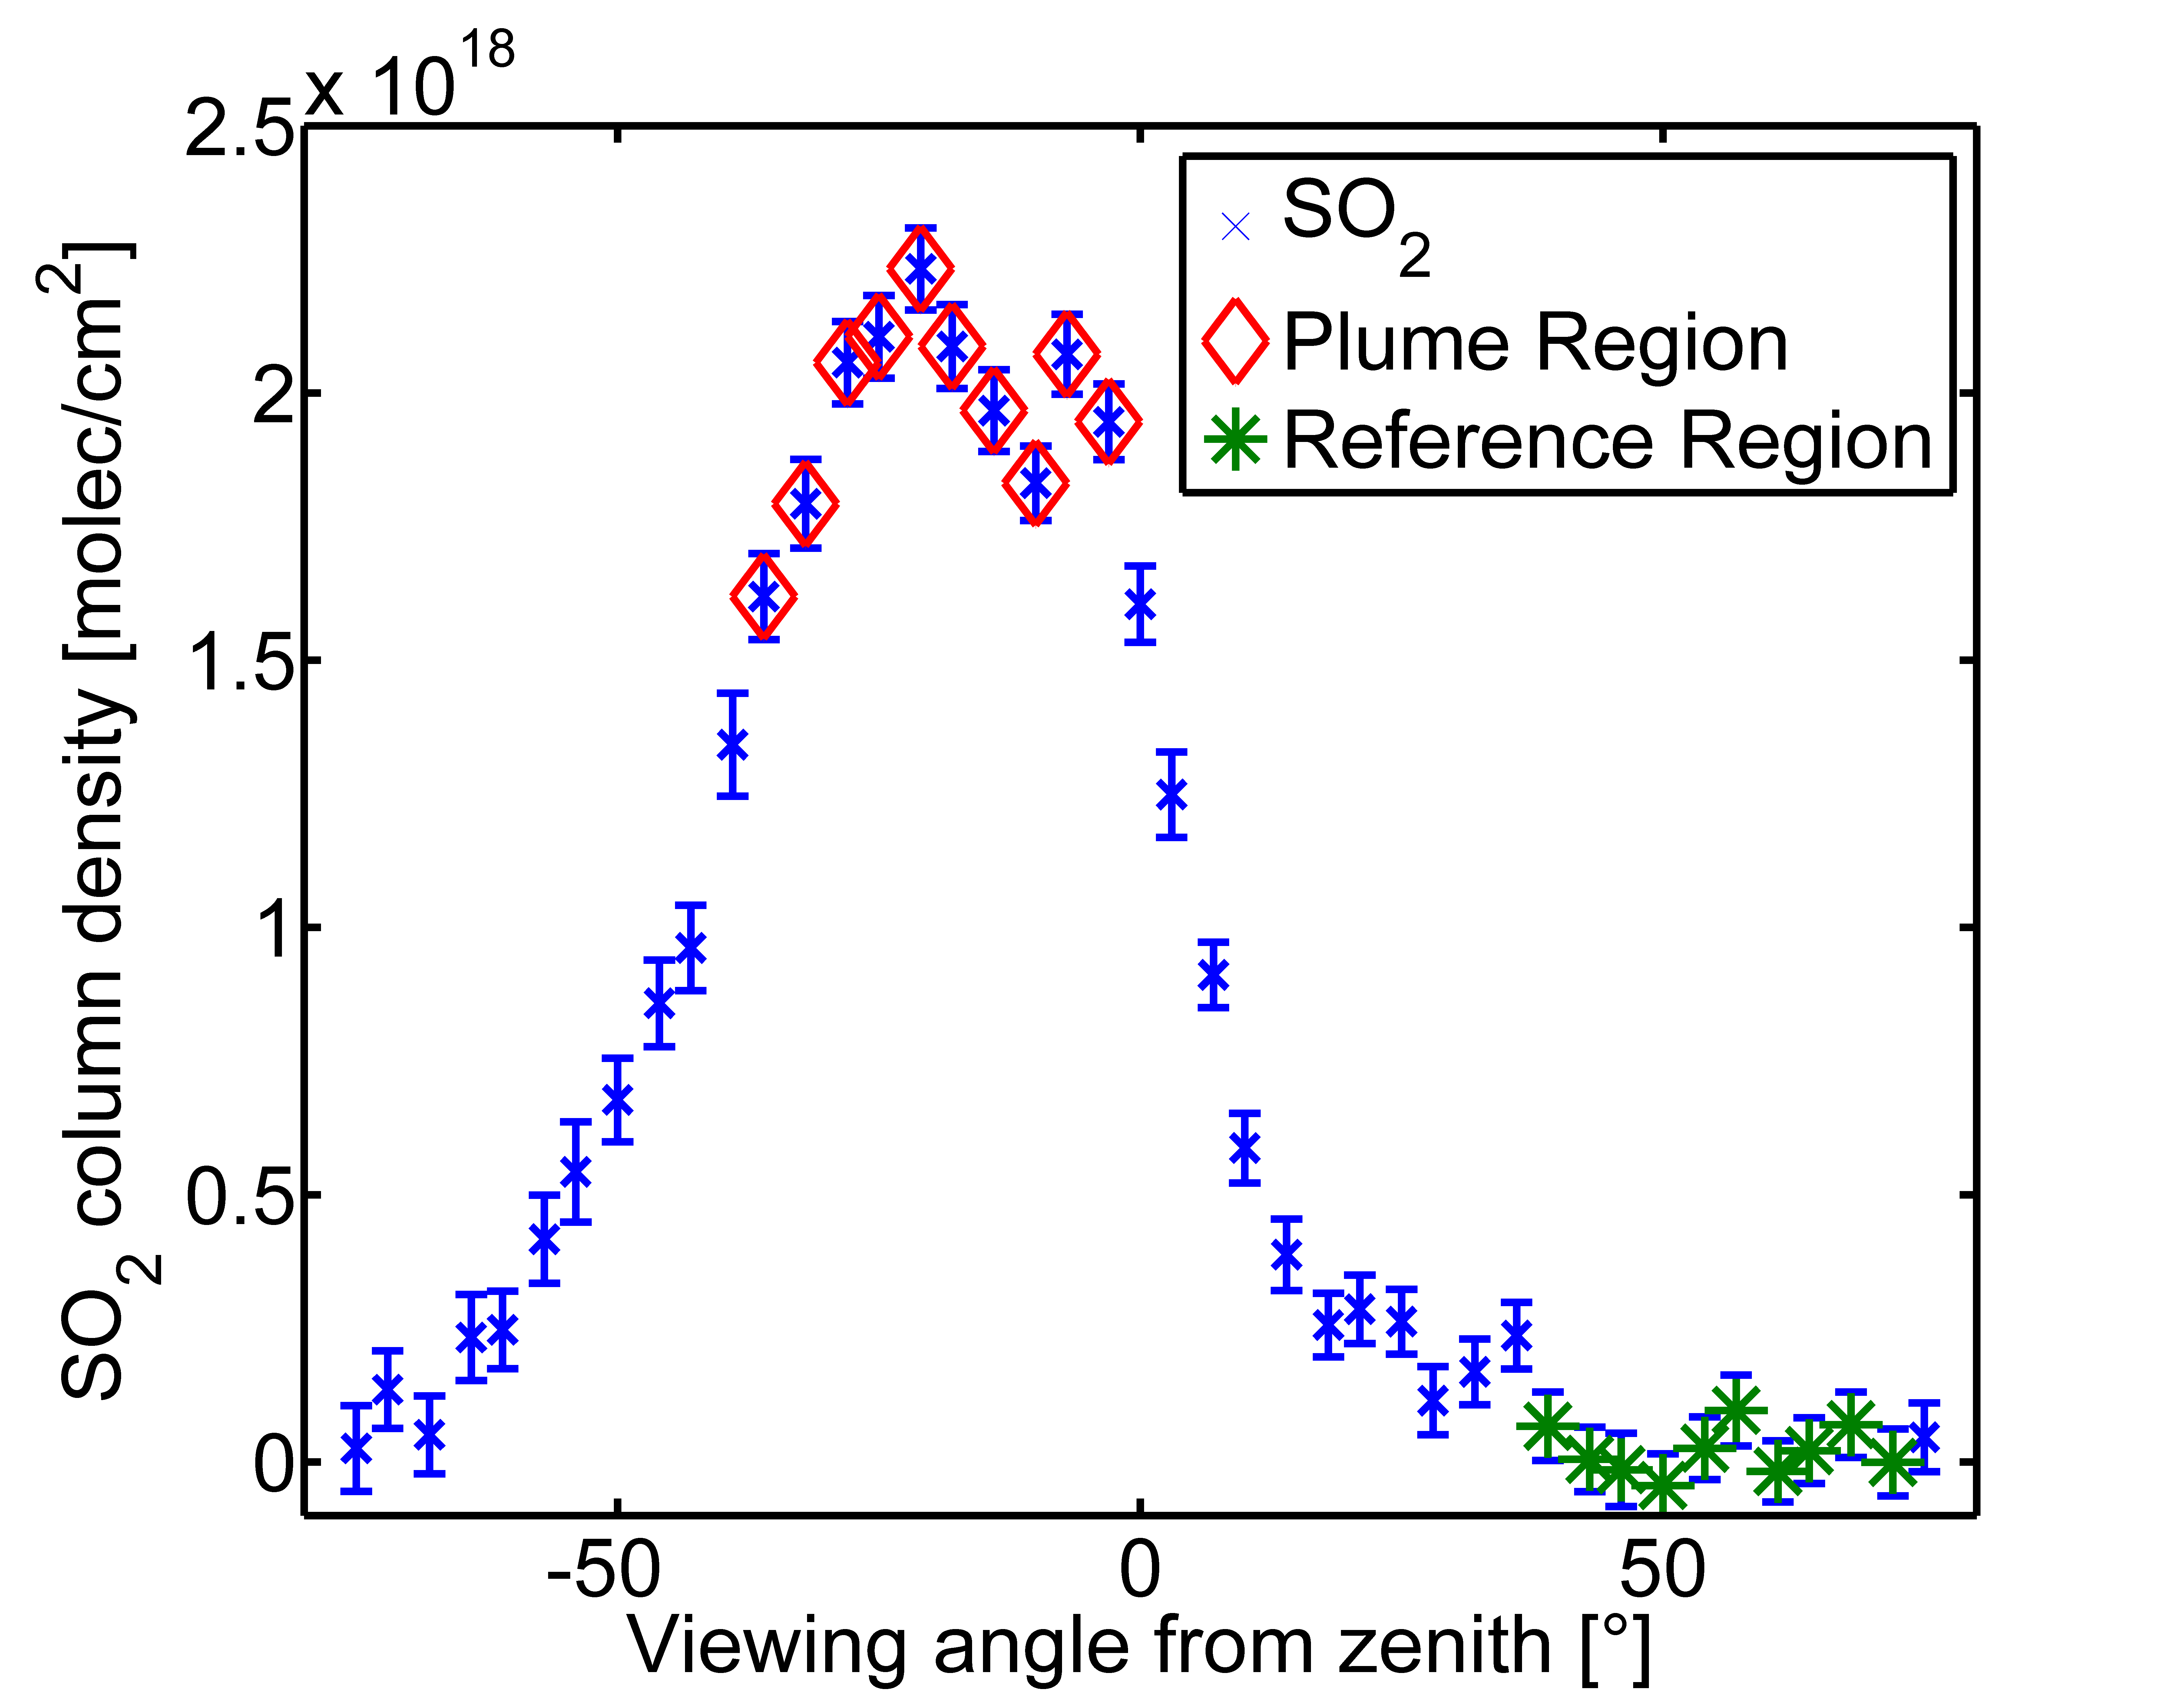
\includegraphics[width=0.53\textwidth]{Bilder/Simon/Bilder_Tung/SO2_Scan}}
	\subfigure[ ]{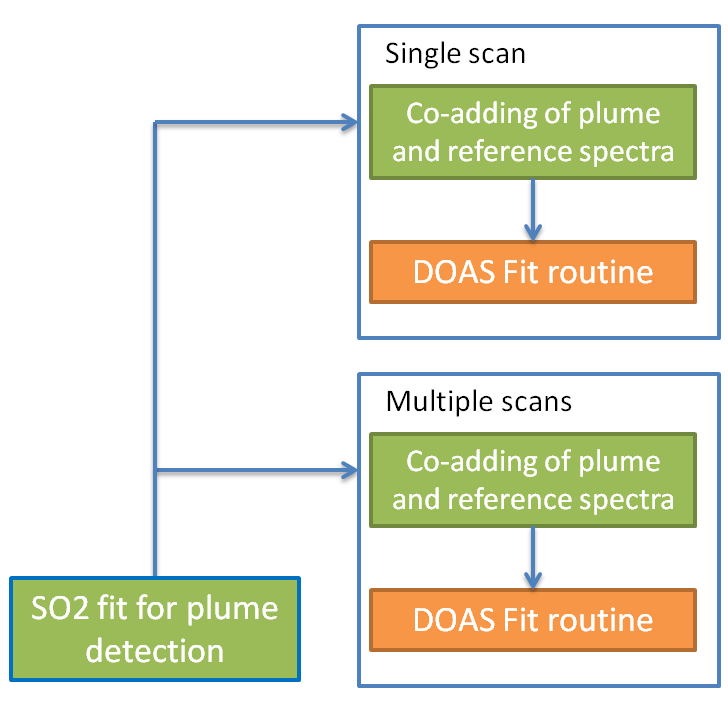
\includegraphics[width=0.47\textwidth]{Bilder/Simon/Bilder_Tung/Algorithm}}
	\caption{(a) \ce{SO2} SCD as a function of the elevation angle. The co-added plume region is marked with red diamonds, and the co added reference region with green stars. From \cite{WarnachSimon}. (b) Flow chart of the \ce{BrO}  and \ce{SO2} evaluation. From \cite{lubcke2014optical}.}
	\label{fig:algorithm}
\end{figure}
\Cref{fig:algorithm} (b) shows the routine of adding multiple spectra of consecutive measuring times. In the following the spectra resulting from the multi adding technique will be referred to as "Multi Add Spectra". The algorithm for co-adding is visualized in \Cref{fig:algorithm} (b) was invented by \citet{vogel2011volcanic} and \citet{lubcke2014bro}. At Tungurahua periods with significant degassing have a mean temporal resolution of 19 and up to 45 "Multi Add Spectra" per day (resulting from three instruments)\\

The mean standard deviation of BrO SCD is about $2.6\cdot10^{13} \frac{molec}{cm^{2}}$. Hereby the standard deviation is estimated as 2 times the DOAS fit error of the multi-scan BrO fit \citet{Stutz96} \\
%
The SO2    detection limit is in the order of $6\cdot10^{16}\frac{molec}{cm^{2}}$.\\
%
Taking the \ce{BrO}/\ce{SO2} molar ratios if the column densities are close to zero yields unpredictable and unrealistic results. 
Thus, spectra measured in a thin volcano plume need to be excluded.
This could be achieved by setting a \ce{BrO} or/and a \ce{SO2} threshold. A reasonable \ce{BrO} threshold needs to be at least in the order of the DOAS fit error. The BrO detection limit can be enhanced by a daily averaging, then one gets a detection limit of BrO$_{DT}=\frac{2.6\cdot10^{13}}{n}\cdot\frac{molec}{cm^{2}}$ (n: number of Multi Add Scans per day, the minimum amount is four): However most BrO SCDs are below the detection limit.
Rejecting all BrO SCDs below the detection limit leads to an drastical decreases of data points since only the high BrO SCDs will be maintained and thus to systematic elevated \ce{BrO}/\ce{SO2} ratios  \citep{lubcke2014bro}.\\
%
The other possibility is to set an \ce{SO2} threshold to ensure only measuring in strong degassing periods. In this thesis an \ce{SO2} threshold (plume limit) of $7\cdot 10^{17} \frac{\text{molec}}{\text{cm}^2}$ is used for the selection of spectra for the evaluation of the \ce{BrO}/\ce{SO2} ratio. \\
%
Within the data above a \ce{SO2} plume limit of $7\cdot 10^{17} \frac{\text{molec}}{\text{cm}^2}$ the maximum detection limit of the BrO/\ce{SO2} ratio is estimated as $(BrO/SO2)_{DT}    =    \frac{\ce{BrO}_{DT}}{SO2_{thres}}=\frac{4    }{\sqrt{n}}\cdot10^{-5}     \leq     1\cdot10^{-5}$.
A plume limit of $7\cdot 10^{17} \frac{\text{molec}}{\text{cm}^2}$ is a high threshold for the column density. However, this approach assures that only strongly significant gas amounts are accounted \citep{lubcke2014bro}. Choosing the \ce{SO2} threshold in this way is a compromise getween a low BrO/\ce{SO2} detection limit and a sufficient amount of data.\\
\begin{figure}
	\centering
	\subfigure{    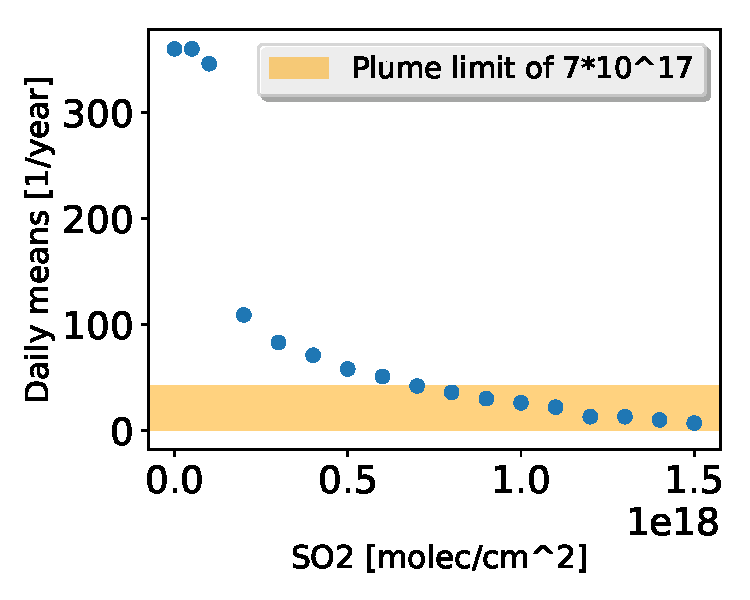
\includegraphics[width=0.49\linewidth]{Bilder/tungpercentage_minSO2}}
	\subfigure{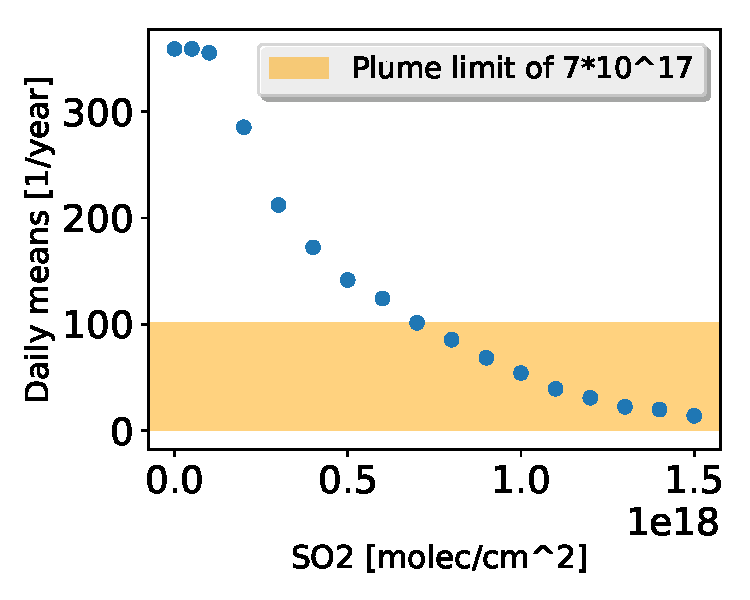
\includegraphics[width=0.49\linewidth]{Bilder/percentage_minSO2}}
	\caption[The ce{SO2} SCD  as a function of the decrease of the amount of daily means amount above the plume limit. Data of Tungurahua and Nevado del Ruiz.]{The ce{SO2} SCD  as a function of the decrease of the amount of daily means amount above the plume limit. The \ce{SO2} SCDs below the actual plume limit of 7$\cdot10^{17}\,\frac{\text{molec}}{\text{cm}^2}$ are marked with a yellow shade. Left: Data of three instruments at Tungurahua. Right: data of two instruments at Nevado del Ruiz.}
	\label{fig:percentageminso2}
\end{figure}
Increasing a plume limit leads to a decrease of usable data. The amount of usable  daily means as a function of the plume limit is shown in \Cref{fig:percentageminso2}. A plume limit of 7$\cdot10^{17}\frac{\text{molec}}{\text{cm}^2}$ leads to a ratio of usable data of approximately 10\%.


\section{Retrieval of absolute slant column densities\label{Chap:Cont}}

At the volcano the atmospheric background levels in \ce{SO2} are negligible, thus one can interpret the dSCDs as SCDS. However, this is not the case if any volcanic trace gases are contaminating the reference spectrum.
The conventional evaluation is based on the assumption, that the reference is free of volcanic gases. This assumption was checked by using a volcanic gas free a high-resolution solar atlas spectrum (see below) to evaluate the reference (\cite{lubcke2014optical}; \cite{salerno2009novel}). In some reference spectra, absorption structures of \ce{SO2}  different from zero are found. This can be a result of spectrographic problems or of a non-negligible amount of volcanic trace gases in the reference region. However, the result is an underestimation of the gas amount by the conventional NOVAC-evaluation.
In ca. 10\% of the data, the reference spectrum is found to be contaminated with volcanic trace gases.
This could happen if, for example, the volcanic plume of the day before extends over the whole scan area as a consequence of windless conditions.
In consequence, the reference is contaminated with volcanic trace gases. Thus, the gas amount is underestimated by the conventional NOVAC-evaluation: In \Cref{fig:contaminated} an example from April 2011 (Tungurahua) where the reference region is contaminated by volcanic trace gases is shown. The blue \ce{SO2} curve shows the calculations with the NOVAC-evaluation, but since there is still \ce{SO2} in the reference region, the assumption, that the \ce{SO2} amount could be set to zero in the reference region is wrong. The red curve shows the \ce{SO2} curve, retrieved with a solar atlas spectrum as reference, which lies significantly above the NOVAC -curve.\\
\\    
%
\begin{figure}
	\centering
	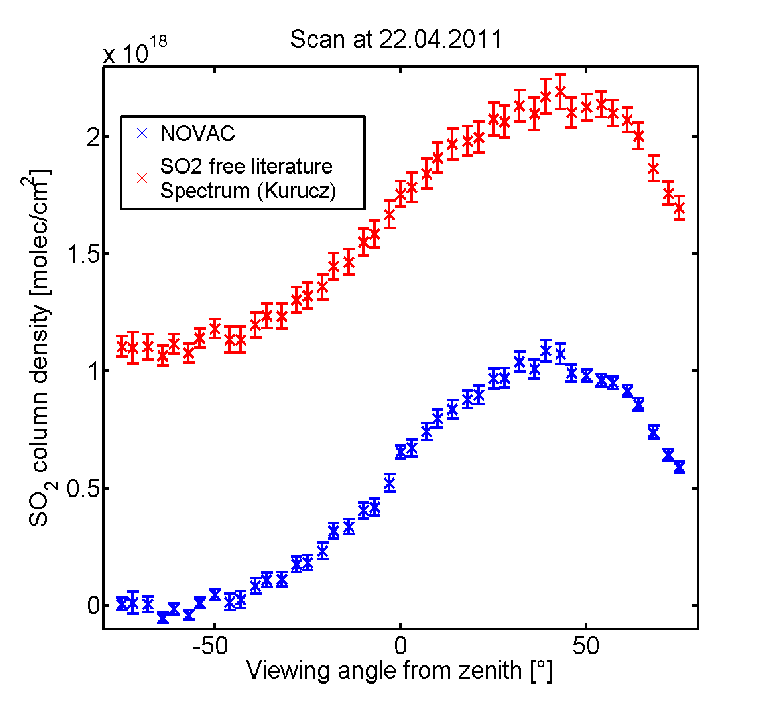
\includegraphics[width=0.7\linewidth]{Bilder/contaminated}
	\caption{Scan with a contaminated reference spectrum from April 2011. From \cite{WarnachSimon}}
	\label{fig:contaminated}
\end{figure}
\\
If the reference region for any reason is
contaminated by volcanic trace gases, there are two possibilities: excluding the contaminated data from the evaluation or the reference spectrum has to be
replaced by a volcanic-gas-free reference. Alternative spectra are a
theoretical solar atlas spectrum or a volcanic-gas-free reference
spectrum recorded by the same instrument at another time.\\
A further possibility is to assume, that contamination only occurs for \ce{SO2}, but not for BrO due to the smaller lifetimes of BrO, thus it is possible to use the Solar atlas spectrum for the \ce{SO2} evaluation, but the reference, recorded by the NOVAC-instrument at the same time for the BrO retrieval. Hereby the assumption, that BrO is not contaminated need to be proved. \\
%
\\
%
In the following, I will discuss the two alternative reference spectra.
%
\subsection*{Evaluation using a Solar Atlas spectrum \label{kuruz}}
An alternative for choosing the region with the lowest column density as reference region is to use a theoretical high-resolution solar atlas spectrum as reference \citep{chance2010improved}.
The use of a theoretical solar atlas spectrum as a reference which is completely volcanic-trace-gases-free was first proposed by \cite{salerno2009novel} and evolved by \citep{lubcke2014bro}.
The advantage of using a solar atlas spectrum as reference is, that it is sure that it is not affected by past or current volcanic gas emissions. Thus, it allows for a retrieval of the absolute trace gas SCDs in the volcanic gas plume. The disadvantage is, that using a solar atlas spectrum comes along with a drawback of precision: The spectral resolution of the theoretical solar atlas spectrum is much  higher than of the NOVAC instruments. Therefore the instrument functions would need to be perfectly modeled and added to the retrieval. This is not straightforward, because the instrumental line-shape varies over the wavelength region and is also mathematically often not perfectly described by a simple approach like Gauss, Lorentz,..etc.\\ 
The reduction of precision is acceptable for the
\ce{SO2} retrieval but not suitable for a \ce{BrO} retrieval because then most data would be below the detection limit.\\
%
\\
%
Possible contaminations can be checked
by a theoretical solar atlas spectrum to evaluate the \ce{SO2} amount in the reference.\\

%
\subsection*{Evaluation using a spectrum of the same instrument}
An alternative reference spectrum could be a volcanic-gas-free reference
spectrum recorded by the same instrument at a different time. When using such a reference several problems occur:\\
As described in \cref{NOVAC} the instruments used in NOVAC do not include features like temperature stabilization. Due to that, the measurements are not independent of external parameters. 
So it is necessary to choose a reference recorded at similar conditions with respect to meteorology and radiation as well as in the temporal proximity due to instrumental changes with time and ambient conditions. Ideally, the external conditions should be equal to the conditions at the time when the plume was recorded.\\
%
When performing the evaluation with the Solar Atlas Spectrum as reference, finding the instrument function occur to be a central challenge. If the instrument function for the solar atlas spectrum is found the function is typically used for a few years This could lead to higher errors due to a gradual worse matching instrument function.
Using the reference of the same instrument but recorded at another day, leads also to problems caused by different instrument functions, but compared to the calculated instrument function used for the evaluation with the solar atlas spectrum those differences in the instrument function could be smaller.
\\
In this work, I combine both options in order to
achieve both, enhanced accuracy but still maximum possible precision of
the \ce{SO2} and \ce{BrO} retrievals. So I use the solar atlas spectrum to check for 
contamination and a reference spectrum recorded in temporal proximity by the same instrument as reference.\\
\begin{figure}
	\centering
	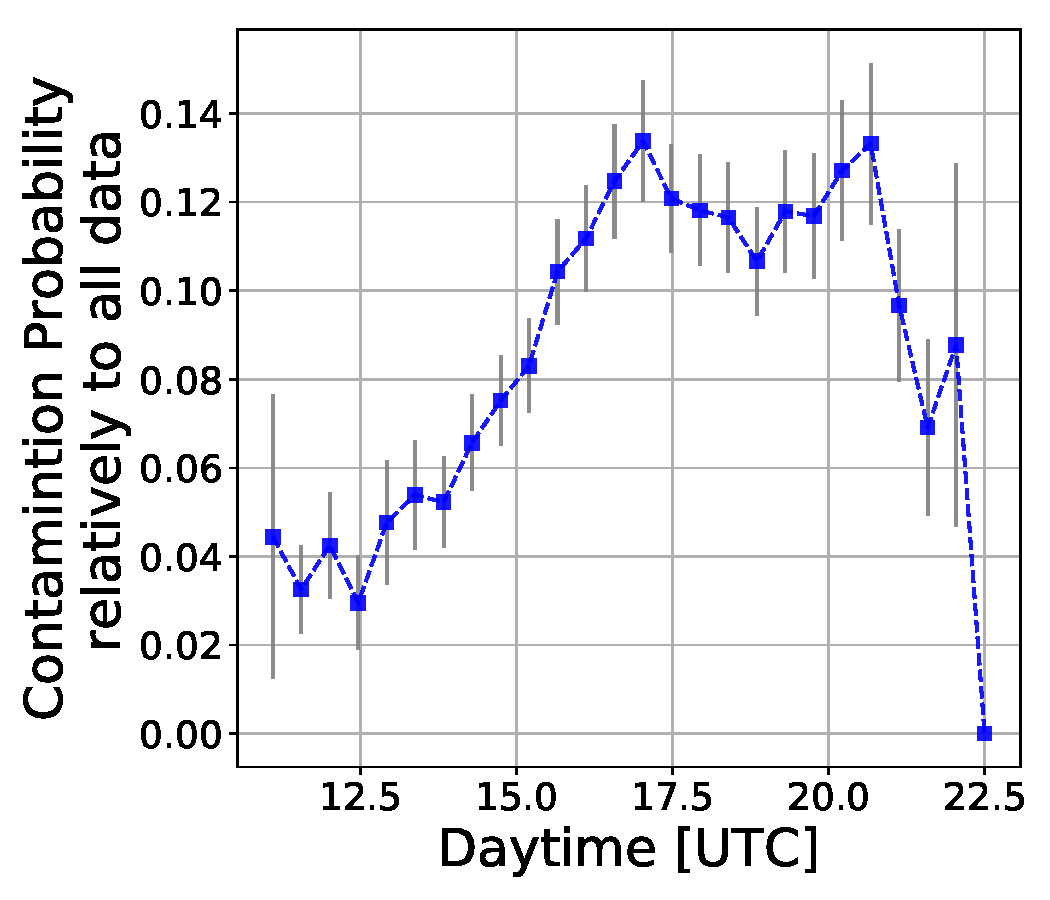
\includegraphics[width=0.5\linewidth]{Bilder/ConProb}
	\caption[The possibility of contamination relatively to all not contaminated data recorded at the same time as a function of the daytime. The data are taken from the Nevado del Ruiz volcano.]{ The possibility of contamination relatively to all not contaminated data recorded at the same time as a function of the daytime. The probability is calculated by dividing the number of contaminated scans recorded at a specific daytime by the amount of not contaminated data recorded at the same daytime. The square root of the data amount is taken as the error, the visualized error is then calculated by using error propagation. The local time can be calculated from the daytime as UTC-5h. The data are taken from the Nevado del Ruiz volcano.}
	\label{fig:conprob}
\end{figure}
The probability of contamination changes with the daytime as can be seen in \cref{fig:conprob}. In the Morning the probability of contamination is much lower than at noon. Thus one can conclude that the conditions on the day favor the occurrence of contamination more than the conditions at night. The decrease of contamination in the evening can be a result of fewer data and is therefore not significant.

If contamination occurs it is possible to choose a new reference from a list of gas-free alternative references. In theory, for ideal instruments, all references should lead to
the same results for the gas retrievals. But instruments are imperfect (see Chapter
4) thus the reference needs to be chosen carefully in order to ensure reliable results.\\
%
\\

\subsection{Contamination of the plume}
As discussed above it might occur, that the reference is contaminated for example by the plume of the day before.
If that happens, the gas amount is underestimated by using a contaminated reference. But another possibility is, that the plume itself is also contaminated. This might be the case if the volcanic gas of the volcano is not taken away by the wind, but accumulates at the instrument. If this is the case, using another reference would lead to an overestimation of the column density of gases. With the data retrieved by the NOVAC instruments, it is very difficult to discover whether the plume is contaminated or not. \\
%
%Thus using a gas-free reference in order to get rid of the contamination problem is arguable because it does not consider contamination of the plume. Moreover, I do not consider the different lifetimes of \ce{SO2} and BrO. This leads to a faster depletion of BrO.\\
%
\begin{figure}
	\centering
	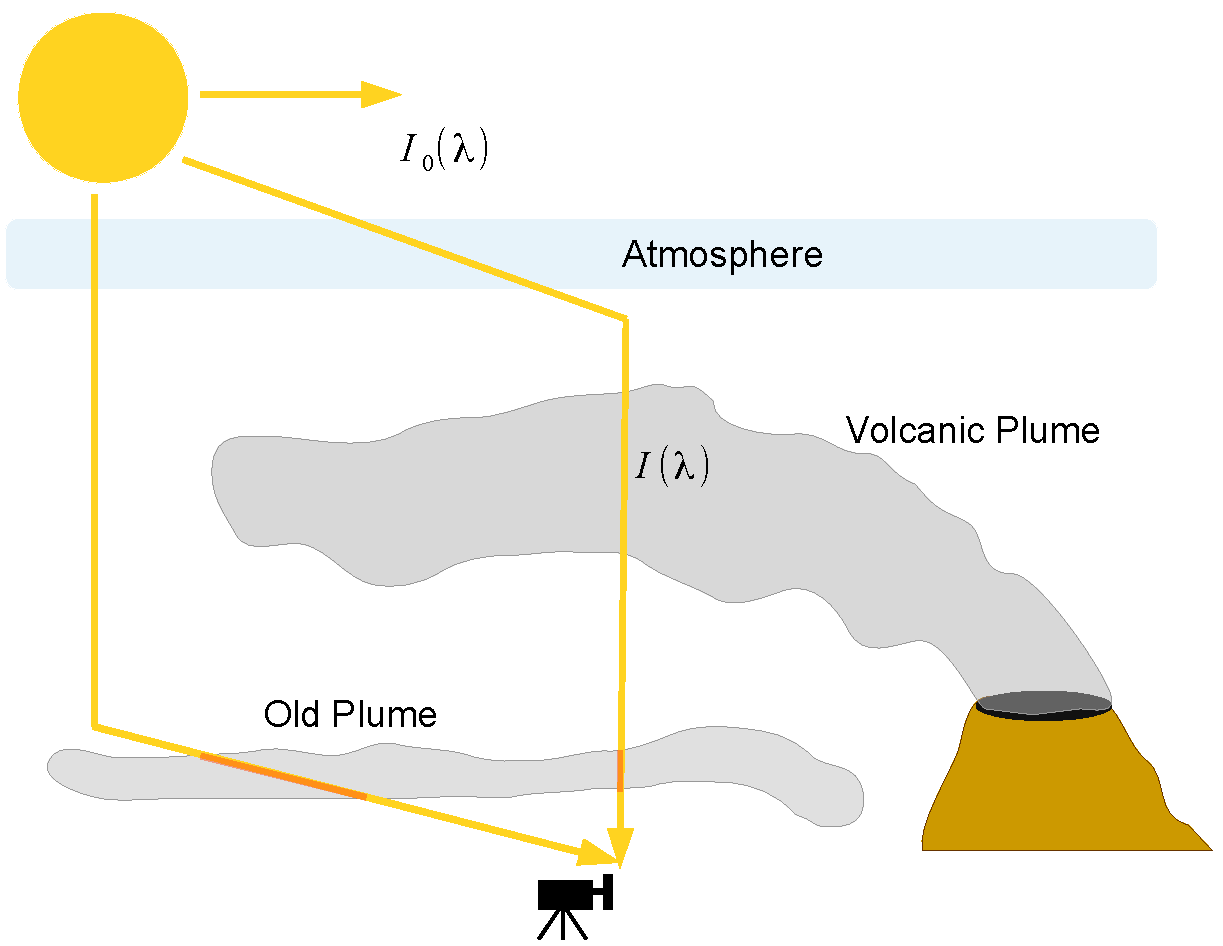
\includegraphics[width=0.7\linewidth]{Bilder/Contaminationplume}
	\caption{Visualization of the contamination of the plume. Due to a lack of wind the old plume sinks down an accumulates
		above the instrument. The light path trough the old plume is longer when recording the reference spectra (orange).}
	\label{fig:contaminationplume}
\end{figure}
\begin{figure}
	\centering
	\subfigure{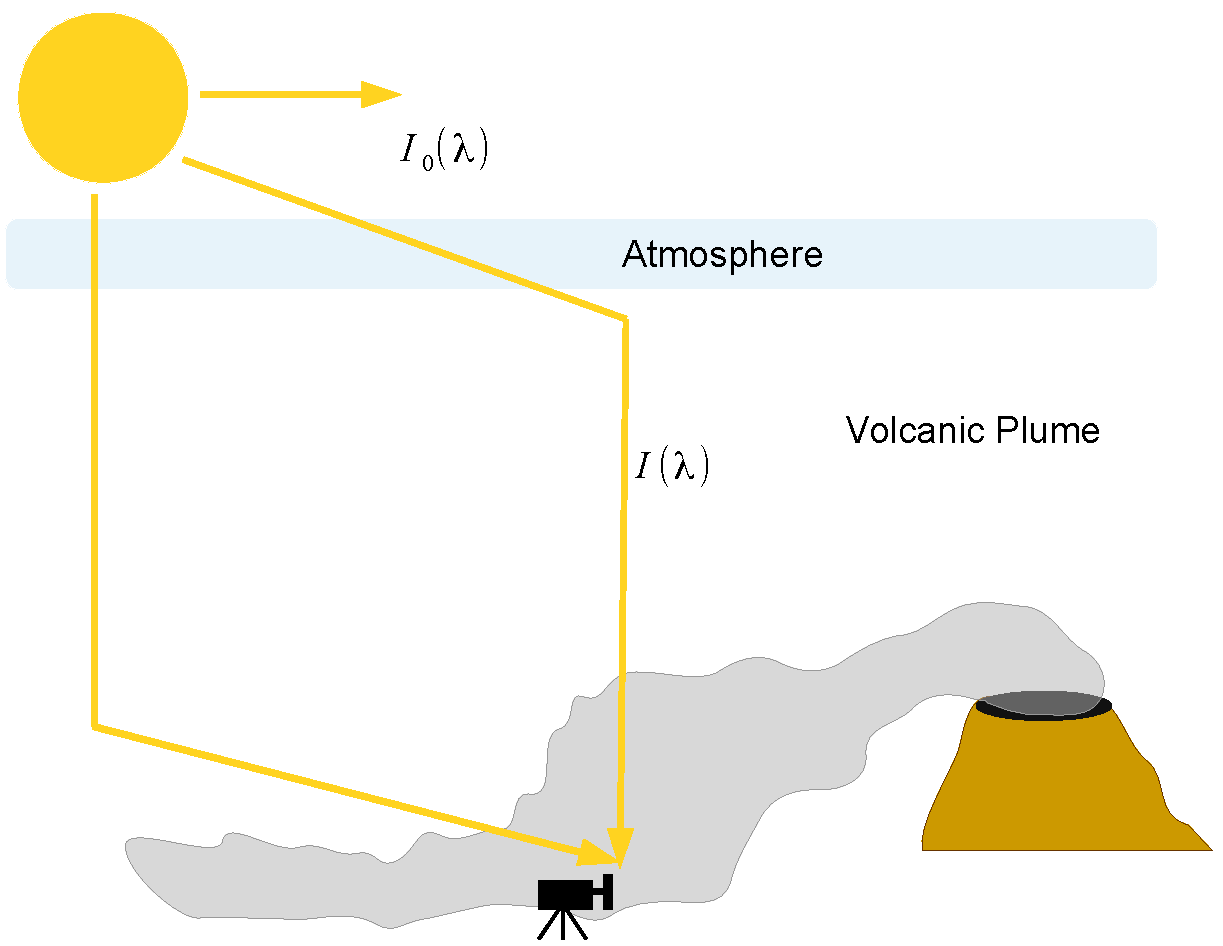
\includegraphics[width=0.49\linewidth]{Bilder/Contaminationplumeinstrinplum}}
	\subfigure{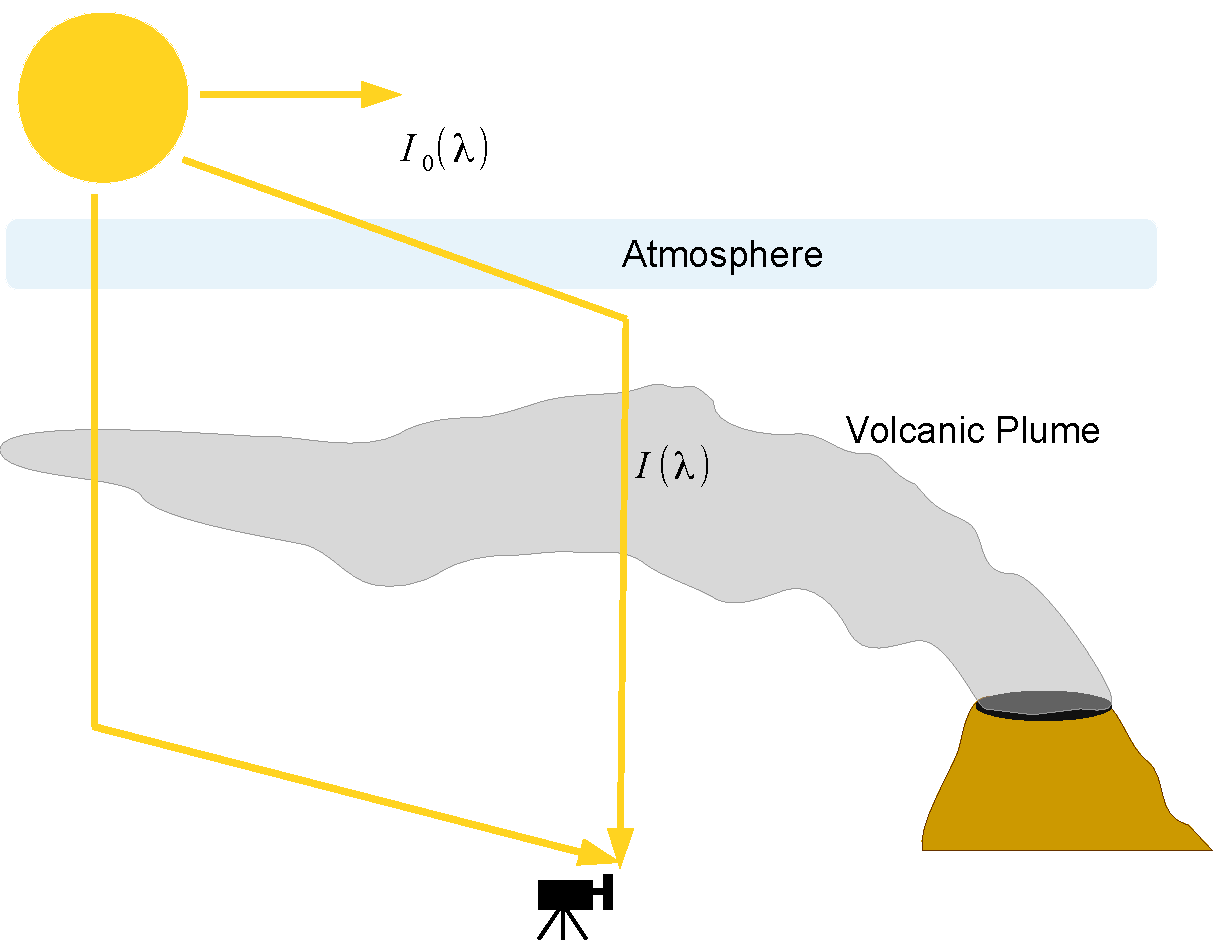
\includegraphics[width=0.49\linewidth]{Bilder/Contaminationplumewideplume}}
	\caption[Visualization of possible scenarios for contamination]{Visualization of possible scenarios for contamination. Left: the plume sinks in a way that the instrument is within the plume, therefore, all elavation angles will contain volcanic trace gases, while the plume is not additionally contaminated. Right: the plume covers the hole sky, thus all elvation angles "see" volcanic trace gases. }
	\label{fig:contaminationplumewideplume}
\end{figure}
%
Plume contamination could occur in a scenario described by  \cref{fig:contaminationplume}.
This might be the case if the volcanic gas of the volcano is not taken away by the wind, but accumulates in the vicinity of the volcano and thus is seen by the instrument. In such a scenario, using a contamination free reference recorded at another time would lead to an overestimation of the gas column densities in the plume.\\
This is one possible occurrence of contamination. As it can be seen gas of the old plume affects the measurement of the reference and the plume. However, for this example, the influence on the measurement of the reference is much larger since the light path through the old plume (colored orange in \cref{fig:contaminationplume}) is longer for the reference than for the measurement of the volcanic plume. Thus, the gas amount is underestimated by not using a gas-free reference, but might be overestimated if a gas-free reference spectrum is used.
The real gas amount might be between the measured amount with and without using a reference measured at another time.\\
%The contamination setup could differ from \cref{fig:contaminationplume}. This would lead to different results. However, the reference region is in most cases at a larger elevation angle than the plume. Thus, the assumption that the light path through the old plume is in average longer for the reference, if both, reference and plume are contaminated.\\
%
With the data retrieved by the NOVAC instruments, it is very difficult or even impossible to discover whether the plume is contaminated or not. \\
\\
\\
\begin{figure}
	\subfigure{
		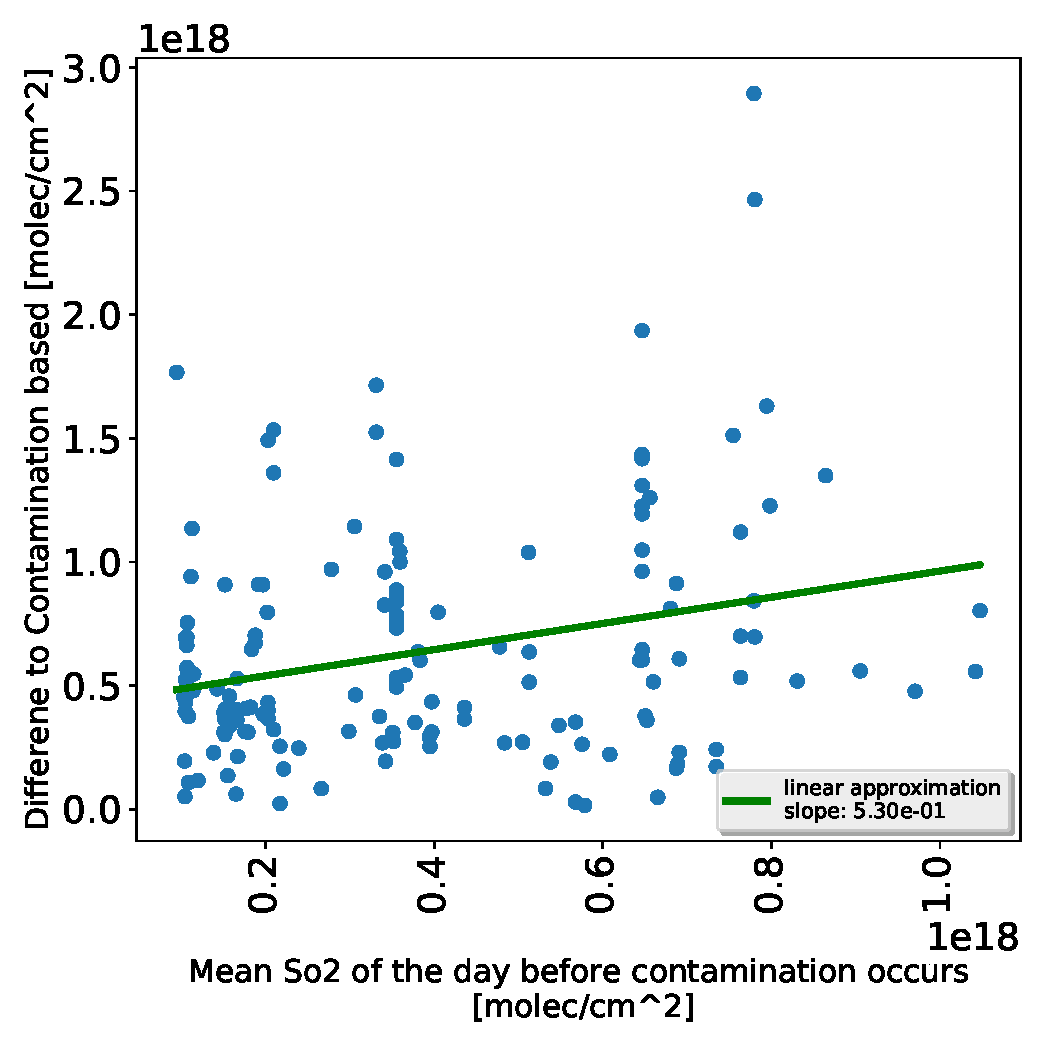
\includegraphics[width=0.5\linewidth]{Bilder/contaminationdependency_so2}}
	\subfigure{
		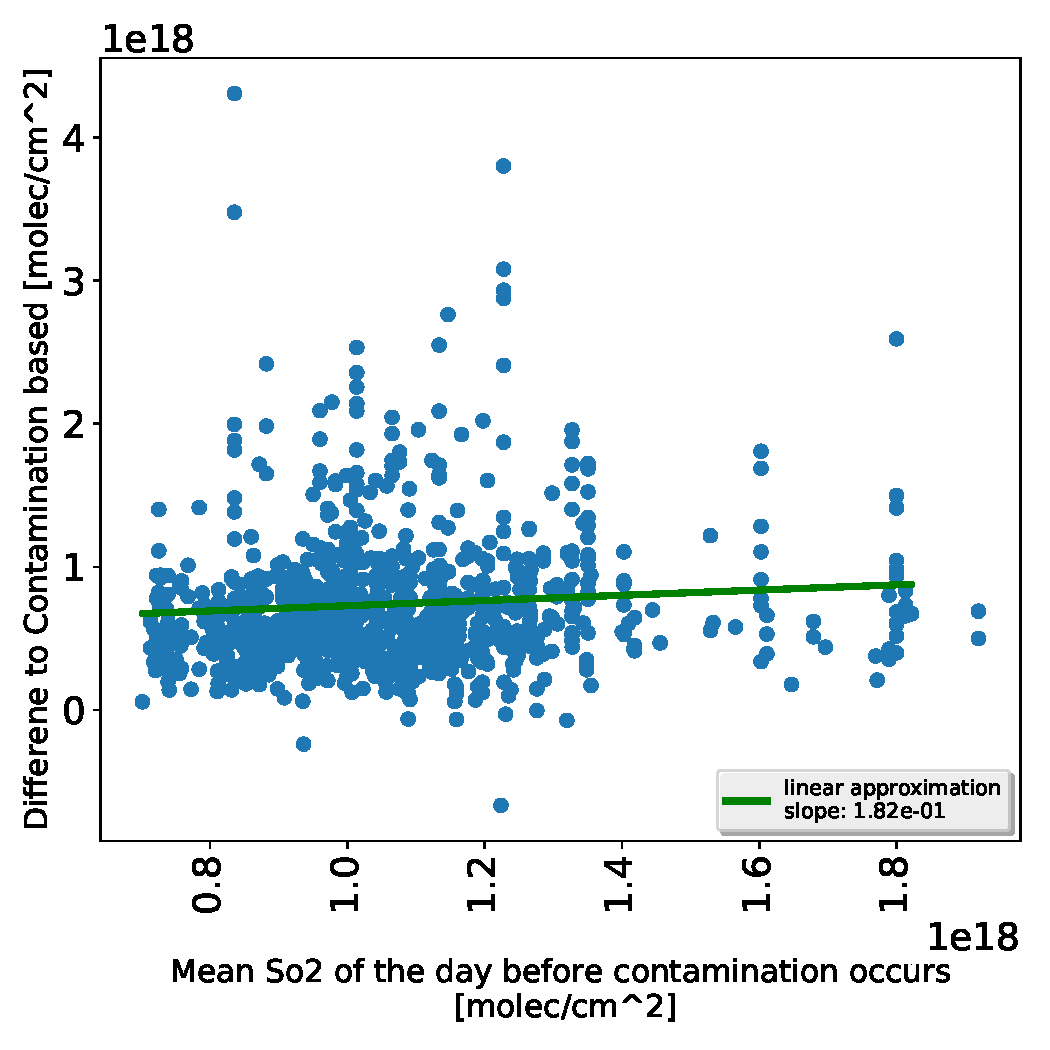
\includegraphics[width=0.5\linewidth]{Bilder/contaminationdependency_so2_Nevad}}
	\caption[The strength of contamination as function of the mean \ce{SO2} column density (daily mean) of the day before. Data from Tungurahua and Nevado Del Ruiz.]{The strength of contamination as function of the mean \ce{SO2} column density (daily mean) of the day before. The strength of contamination is defined as the difference in \ce{SO2} SCD  when evaluation with an alternative reference, or neglect the contamination. Left: data from Tungurahua. Right: data from Nevado Del Ruiz. }
	\label{fig:contaminationdependencyso2}
\end{figure}

If the contamination is a result of strong emissions of the day before, a dependency of the strength of contamination on the emission of the day before could appear. 
The mean \ce{SO2} SCDs of a day (daily mean) could be used as a proxy for the total emission. The strength of contamination can be calculated as the difference between the evaluation for \ce{SO2} with a contaminated reference recorded at the same time as the plume spectrum was recorded and using a gas-free reference. Such a plot is shown for Tungurahua and Nevado del Ruiz in \cref{fig:contaminationdependencyso2}. Even though both plots show a slight increase in contamination strength with the mean amount of \ce{SO2} of the day before, the increase is not significant. Another possible proxy for the \ce{SO2} emission would be the maximum \ce{SO2} SCD of the day before contamination occurs. However, taking the maximum does not lead to a more significant relation between the emission and the strength of contamination. \\
Thus the \ce{SO2} emission is, if it influences the possibility of contamination, not the only significant factor. To further examine the reasons for contamination the wind conditions should be studied in particular. 
%\textcolor{red}{hier waere es gut noch andere parameter zu testen - wie in Luebcke et al, zum beispile als funktion von Wind geschwindigkeit,..   Für NdR kann ich die Meteorologischen Daten ab 2014 beisteuern.}
\\
However, this thesis is built on the assumption, that the plume is free of additional contamination. %\textcolor{yellow}{Nicole hat hier noch fragen, was ?}. 
In the following, I discuss how to automatically determine an optimal reference from another scan.



